% ============================================================================
% CAPÍTULO 4 — RESULTADOS
% ============================================================================
\chapter{Resultados}
\label{cap:resultados}

Este capítulo reporta os resultados de três conjuntos de dados (estudo
piloto, Experimento A e Experimento B), todos gerados com o modelo
\texttt{llama3.1:8b} (seção \ref{sec:selecao-modelo}), com 300 agentes
cada, seguidos das rodadas da análise de robustez e generalização.
Antes deles, a seção \ref{sec:resultados-sorteio} verifica se o sorteio
dos perfis de personalidade ficou equilibrado e independente entre os
traços, condição para que os resultados seguintes possam ser atribuídos a
cada traço. A seção \ref{sec:resultados-piloto} reporta o \textbf{estudo piloto}
(instrumento BFI-10), etapa inicial que motivou a escolha do modelo e
produziu o primeiro indício do achado central deste trabalho. A seção
\ref{sec:resultados-exp-a} reporta o \textbf{Experimento A}, instrumento
BFI-44, desenho de indução simultânea dos cinco traços. Esta é a
\textbf{análise principal} do trabalho; salvo indicação em contrário,
``os resultados'' referem-se a ela. A seção \ref{sec:resultados-exp-b}
reporta o \textbf{Experimento B}, mesmo instrumento e modelo do
Experimento A, mas com apenas um traço variando por agente: uma
verificação do desenho de indução, não uma segunda análise principal. A
seção \ref{sec:resultados-robustez} reporta a análise de robustez e
generalização (outras temperaturas, novo sorteio de perfis e outros
modelos de linguagem). A comparação entre os quatro modelos de linguagem
testados na seleção do modelo, feita com o BFI-10, está no Capítulo
\ref{cap:metodologia} (seção \ref{sec:selecao-modelo}). Nenhuma seção deste capítulo discute o alinhamento
dos achados com a literatura de referência; essa discussão fica para o
Capítulo \ref{cap:discussao}.

\section{Verificação do sorteio dos perfis de personalidade}
\label{sec:resultados-sorteio}

Como os níveis de personalidade de cada agente foram definidos por sorteio
(seção \ref{sec:desenho-fatorial}), foi verificado se esse sorteio ficou
equilibrado entre os níveis e independente entre os traços. Um sorteio
concentrado em alguns níveis, ou com traços correlacionados entre si,
poderia fazer o efeito de um traço ser atribuído a outro. O estudo piloto e
o Experimento A usaram exatamente o mesmo sorteio (semente 123), de
modo que as verificações a seguir valem para os dois.

\subsection{Equilíbrio entre os níveis}

Em cada um dos cinco traços, cada nível recebeu entre \aleatContagemMin{} e
\aleatContagemMax{} dos \aleatN{} agentes, sem desvio significativo da
distribuição uniforme em nenhum traço (p $\geq$ \aleatPFreqMin; Tabela
\ref{tab:aleat-frequencias} e Figura \ref{fig:aleat-niveis}). A soma dos 5
níveis por agente teve média \aleatSomaMedia{} e desvio padrão
\aleatSomaDP, próximos dos valores esperados para um sorteio uniforme (10
e 1,83). A distribuição também se manteve estável ao longo da geração: os
primeiros e os últimos 150 agentes não diferem em nenhum traço (p entre
\aleatPMetadesMin{} e \aleatPMetadesMax).

% Gerado por analise_aleatorizacao.py -- não editar à mão; rode o script de novo.
\begin{table}[htb]
    \caption{Distribuição dos níveis induzidos por traço (Experimento A e piloto, N=300)}
    \label{tab:aleat-frequencias}
    \centering
    \small
    \begin{tabular}{lccccc}
        \toprule
        Traço & Baixo & Médio & Alto & $\chi^2$ & p-valor \\
        \midrule
        Extroversão & 99 (33,0\%) & 96 (32,0\%) & 105 (35,0\%) & 0,42 & 0,811 \\
        Amabilidade & 102 (34,0\%) & 98 (32,7\%) & 100 (33,3\%) & 0,08 & 0,961 \\
        Consciência & 101 (33,7\%) & 105 (35,0\%) & 94 (31,3\%) & 0,62 & 0,733 \\
        Neuroticismo & 92 (30,7\%) & 112 (37,3\%) & 96 (32,0\%) & 2,24 & 0,326 \\
        Abertura à Experiência & 107 (35,7\%) & 98 (32,7\%) & 95 (31,7\%) & 0,78 & 0,677 \\
        \bottomrule
    \end{tabular}
    \legend{Fonte: dados da pesquisa. Teste qui-quadrado de aderência à distribuição uniforme (100 agentes por nível), 2 graus de liberdade. O piloto usou o mesmo sorteio (semente 123).}
\end{table}


\begin{figure}[htb]
    \caption{Número de agentes por nível induzido em cada traço (Experimento A)}
    \label{fig:aleat-niveis}
    \centering
    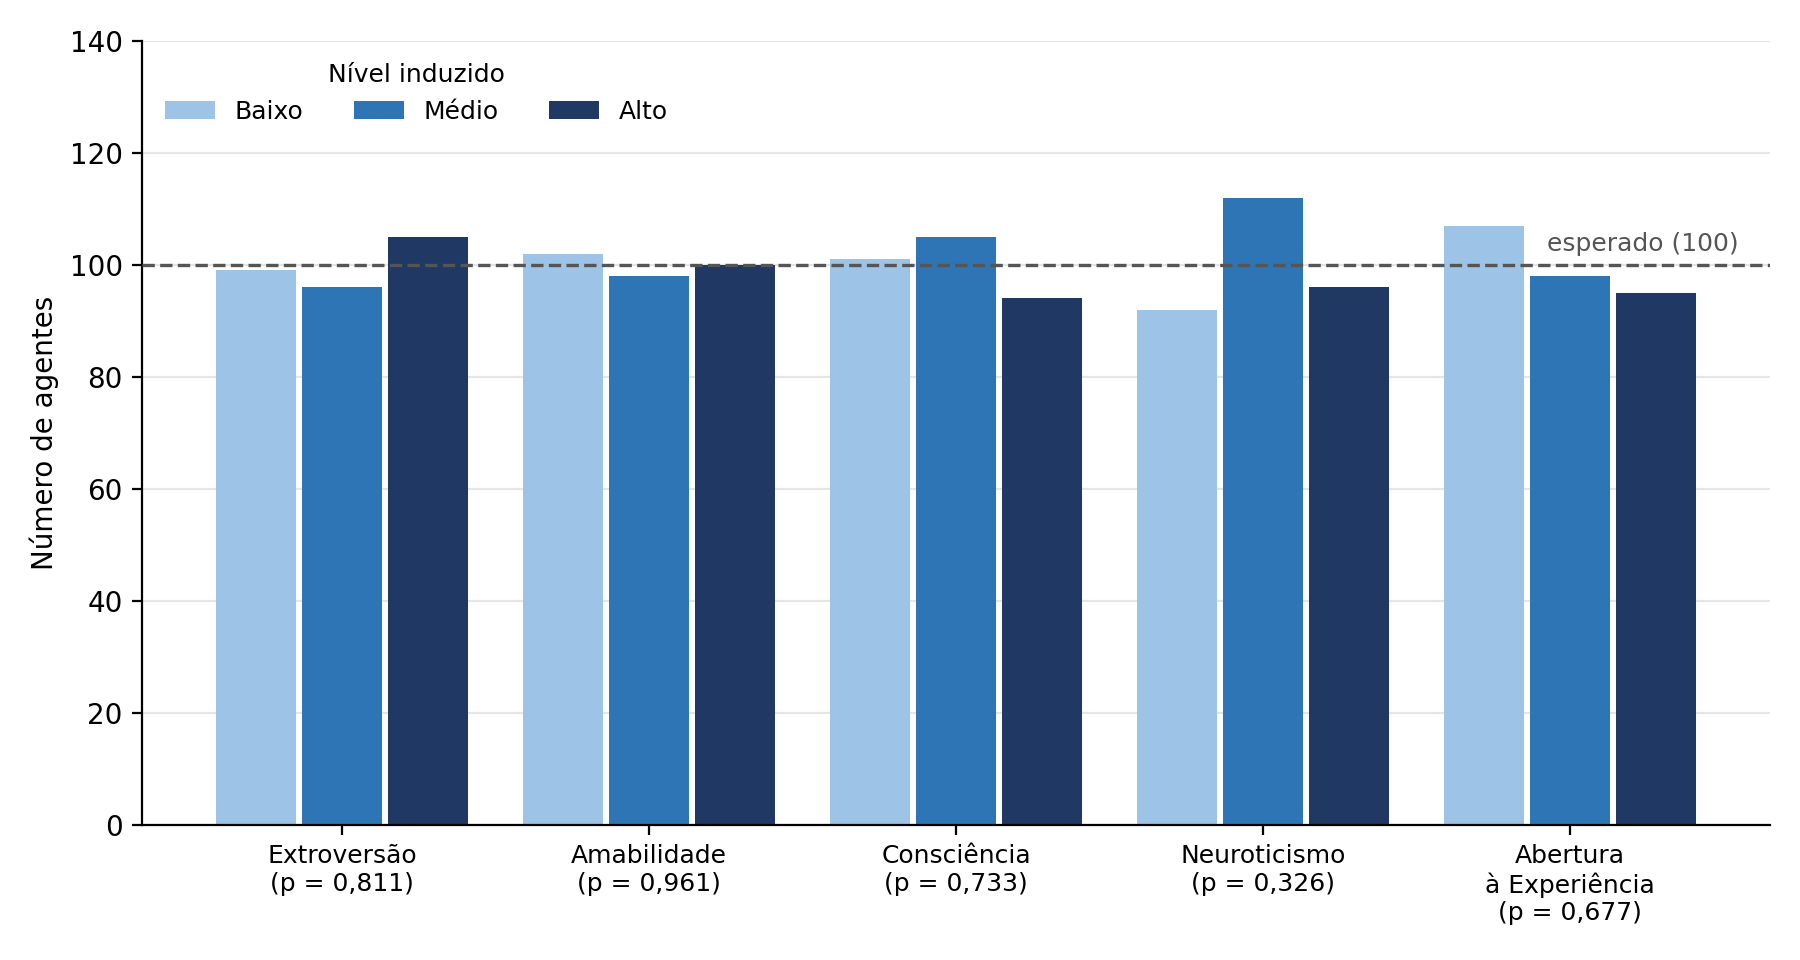
\includegraphics[width=\textwidth]{../resultados/figuras/fig10_aleatorizacao_niveis.png}
    \legend{Fonte: dados da pesquisa. Linha tracejada: contagem esperada em um sorteio uniforme.}
\end{figure}

\subsection{Independência entre os traços}

Nenhum par de traços apresentou associação significativa entre os níveis
sorteados ($|\rho| \leq$ \aleatRhoMax, p $\geq$ \aleatPRhoMin; V de Cramér
$\leq$ \aleatCramerMax; Tabela \ref{tab:aleat-independencia}). Na regressão
OLS com os cinco traços, o fator de inflação da variância ficou entre
\aleatVIFMin{} e \aleatVIFMax, ou seja, sem multicolinearidade entre os
preditores.

% Gerado por analise_aleatorizacao.py -- não editar à mão; rode o script de novo.
\begin{table}[htb]
    \caption{Associação entre os níveis induzidos de cada par de traços (Experimento A)}
    \label{tab:aleat-independencia}
    \centering
    \footnotesize
    \begin{tabular}{lccccc}
        \toprule
        Par de traços & $\rho$ & p ($\rho$) & $\chi^2$ & p ($\chi^2$) & V de Cramér \\
        \midrule
        Amabilidade $\times$ Neuroticismo & +0,103 & 0,075 & 3,50 & 0,478 & 0,076 \\
        Consciência $\times$ Neuroticismo & +0,053 & 0,364 & 1,74 & 0,783 & 0,054 \\
        Extroversão $\times$ Consciência & $-$0,049 & 0,398 & 6,44 & 0,169 & 0,104 \\
        Amabilidade $\times$ Consciência & +0,040 & 0,494 & 1,84 & 0,764 & 0,055 \\
        Extroversão $\times$ Neuroticismo & $-$0,021 & 0,715 & 0,69 & 0,953 & 0,034 \\
        Extroversão $\times$ Amabilidade & +0,015 & 0,790 & 3,81 & 0,433 & 0,080 \\
        Extroversão $\times$ Abertura à Experiência & +0,011 & 0,855 & 2,46 & 0,652 & 0,064 \\
        Amabilidade $\times$ Abertura à Experiência & $-$0,011 & 0,845 & 4,17 & 0,383 & 0,083 \\
        Consciência $\times$ Abertura à Experiência & $-$0,006 & 0,921 & 3,78 & 0,436 & 0,079 \\
        Neuroticismo $\times$ Abertura à Experiência & $-$0,003 & 0,958 & 4,97 & 0,290 & 0,091 \\
        \bottomrule
    \end{tabular}
    \legend{Fonte: dados da pesquisa. $\rho$: correlação de Spearman; $\chi^2$: teste de independência (4 graus de liberdade).}
\end{table}


\subsection{Comparação com sorteios simulados}

Para avaliar se o sorteio obtido é típico do acaso, foram simulados
\aleatNSim{} sorteios com o mesmo desenho. Em todos os indicadores da
Tabela \ref{tab:aleat-montecarlo}, o sorteio obtido ficou dentro da faixa
produzida pelas simulações. O número de combinações distintas de níveis
(\aleatCombUnicas{} das 243 possíveis) é próximo da média simulada
(\aleatCombEsperado); combinações sem nenhum agente são, portanto, uma
propriedade esperada do desenho por sorteio, e não uma falha dele.

% Gerado por analise_aleatorizacao.py -- não editar à mão; rode o script de novo.
\begin{table}[htb]
    \caption{Sorteio obtido vs. 10.000 sorteios simulados}
    \label{tab:aleat-montecarlo}
    \centering
    \footnotesize
    \begin{tabular}{lcc}
        \toprule
        Indicador & Obtido & Simulação \\
        \midrule
        Combinações distintas (de 243 possíveis) & 174 & média 172,4; IC 95\% 163 a 182 \\
        Máximo de agentes com a mesma combinação & 5 & IC 95\% 4 a 7 \\
        Maior $|\rho|$ entre pares de traços & 0,103 & 54,2\% das simulações $\geq$ obtido \\
        Maior desvio de uma contagem em relação a 100 & 12 & 86,9\% das simulações $\geq$ obtido \\
        \bottomrule
    \end{tabular}
    \legend{Fonte: dados da pesquisa. Simulação: 300 agentes, 5 traços, 3 níveis equiprováveis e independentes.}
\end{table}


\subsection{Impacto sobre os resultados}

Se o sorteio tivesse produzido traços correlacionados, o coeficiente de um
traço mudaria ao incluir os demais no modelo. A Tabela
\ref{tab:aleat-impacto} mostra que isso não ocorre: os coeficientes da
regressão simples e da OLS com os cinco traços são muito próximos (Abertura à
Experiência: \aleatAberturaCoefSimples{} e \aleatAberturaCoefMulti), e os
traços significativos são os mesmos nos dois modelos.

% Gerado por analise_aleatorizacao.py -- não editar à mão; rode o script de novo.
\begin{table}[htb]
    \caption{Coeficiente de cada traço sobre o escore IPA: regressão simples vs. OLS com os 5 traços (Experimento A)}
    \label{tab:aleat-impacto}
    \centering
    \small
    \begin{tabular}{lcccc}
        \toprule
        Traço & Coef. simples & p-valor & Coef. OLS (5 traços) & p-valor \\
        \midrule
        Abertura à Experiência & +1,722 & $<$ 0,001 & +1,716 & $<$ 0,001 \\
        Extroversão & +1,165 & $<$ 0,001 & +1,189 & $<$ 0,001 \\
        Consciência & +0,704 & $<$ 0,001 & +0,750 & $<$ 0,001 \\
        Neuroticismo & +0,424 & 0,033 & +0,407 & 0,006 \\
        Amabilidade & +0,164 & 0,392 & +0,094 & 0,511 \\
        \bottomrule
    \end{tabular}
    \legend{Fonte: dados da pesquisa. Variável dependente: escore IPA sem a pergunta 1 (N=300).}
\end{table}


\subsection{Experimento B e pergunta 1 do IPA}

No Experimento B, o traço dominante foi distribuído de forma equilibrada
entre os agentes ($\chi^2$ = \aleatDominanteChi, p = \aleatDominanteP;
Tabela \ref{tab:aleat-exp-b}). O único desequilíbrio está nos níveis de
Neuroticismo quando dominante (p = \aleatNeuroBP), que deixa de ser
significativo após a correção de Bonferroni para os cinco testes (limite
de 0,01). Esse desequilíbrio pode reduzir ligeiramente o poder do teste
de Neuroticismo isolado.

% Gerado por analise_aleatorizacao.py -- não editar à mão; rode o script de novo.
\begin{table}[htb]
    \caption{Distribuição do traço dominante e de seus níveis (Experimento B)}
    \label{tab:aleat-exp-b}
    \centering
    \small
    \begin{tabular}{lccccc}
        \toprule
        Traço dominante & N & Baixo & Médio & Alto & p-valor \\
        \midrule
        Neuroticismo & 69 & 21 & 15 & 33 & 0,026 \\
        Consciência & 63 & 19 & 25 & 19 & 0,565 \\
        Amabilidade & 62 & 21 & 16 & 25 & 0,374 \\
        Extroversão & 57 & 22 & 22 & 13 & 0,241 \\
        Abertura à Experiência & 49 & 13 & 20 & 16 & 0,470 \\
        \bottomrule
    \end{tabular}
    \legend{Fonte: dados da pesquisa. p-valor: qui-quadrado de aderência à uniforme entre os 3 níveis. Distribuição do traço dominante: $\chi^2$ = 3,73, p = 0,443.}
\end{table}


A pergunta 1 do IPA (faixa etária), também sorteada, não se afastou da
distribuição uniforme no Experimento A ($\chi^2$ = \aleatQUmChi, p =
\aleatQUmP). Como as análises usam o escore IPA sem essa pergunta, ela não
interfere nos resultados.

\section{Estudo piloto (BFI-10)}
\label{sec:resultados-piloto}

A Tabela \ref{tab:manipulacao-piloto} e a Figura \ref{fig:manipulacao-piloto}
apresentam a checagem de manipulação do estudo piloto: correlação de
Spearman entre o nível de personalidade induzido (1/2/3) e o escore de
autorrelato do agente no BFI-10, por traço.

\begin{table}[htb]
    \caption{Estudo piloto: correlação entre nível induzido e autorrelato (BFI-10, N=300)}
    \label{tab:manipulacao-piloto}
    \centering
    \begin{tabular}{lccc}
        \toprule
        Traço & $\rho$ & p-valor & Avaliação \\
        \midrule
        Neuroticismo            & 0,838 & $<$ 0,001 & Forte \\
        Amabilidade              & 0,812 & $<$ 0,001 & Forte \\
        Abertura à Experiência  & 0,739 & $<$ 0,001 & Forte \\
        Consciência             & 0,507 & $<$ 0,001 & Forte \\
        Extroversão             & 0,410 & $<$ 0,001 & Moderada \\
        \bottomrule
    \end{tabular}
    \legend{Fonte: dados da pesquisa. Avaliação: forte para $\rho \geq 0{,}50$; moderada para $0{,}30 \leq \rho < 0{,}50$.}
\end{table}

\begin{figure}[htb]
    \caption{Estudo piloto: checagem de manipulação por traço (BFI-10)}
    \label{fig:manipulacao-piloto}
    \centering
    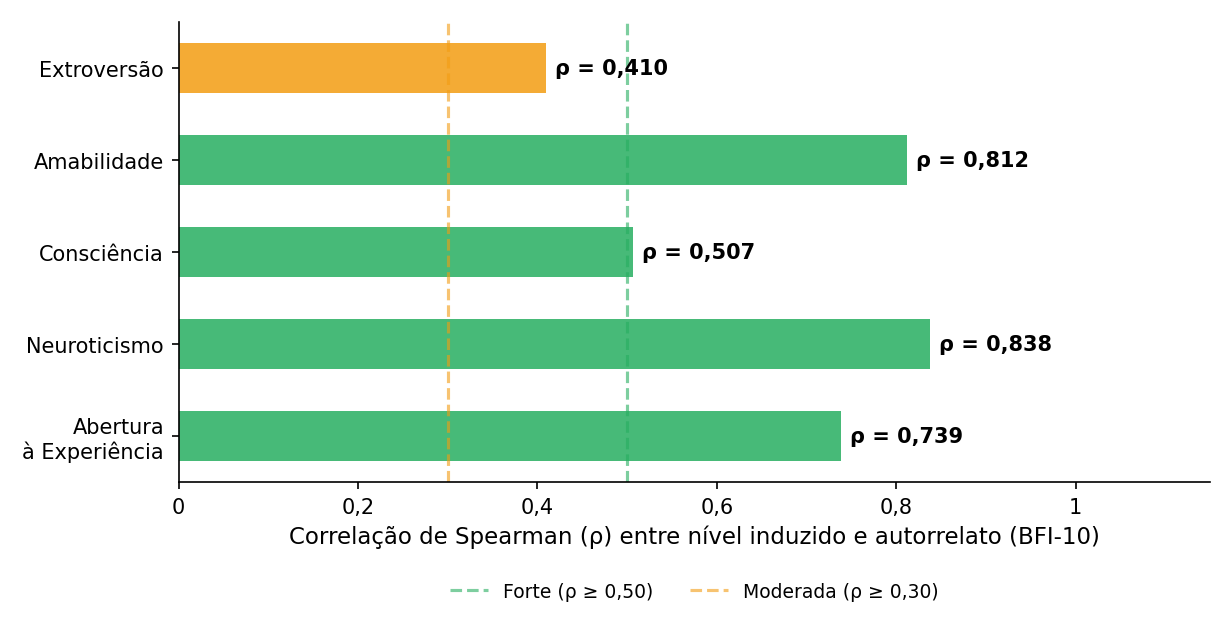
\includegraphics[width=0.8\textwidth]{../resultados/figuras/fig4_manipulacao_piloto.png}
    \legend{Fonte: dados da pesquisa.}
\end{figure}

Todos os cinco traços foram incorporados de forma estatisticamente
significativa; Extroversão foi a mais fraca (ainda assim moderada),
padrão compatível com o viés de discordância em itens de pontuação
reversa descrito na seção \ref{sec:limitacoes-pipeline}.

A Tabela \ref{tab:distribuicao-ipa-piloto} mostra a distribuição do
perfil de investidor obtido, e a Tabela \ref{tab:spearman-ipa-piloto}
(com as Figuras \ref{fig:spearman-piloto} e \ref{fig:boxplots-piloto}) a
correlação entre nível induzido e escore do IPA, por traço.

\begin{table}[htb]
    \caption{Estudo piloto: distribuição do perfil IPA (BFI-10, N=300)}
    \label{tab:distribuicao-ipa-piloto}
    \centering
    \begin{tabular}{lcc}
        \toprule
        Perfil & N & \% \\
        \midrule
        Conservador & 15  & 5\%  \\
        Moderado    & 235 & 78\% \\
        Arrojado    & 50  & 17\% \\
        \bottomrule
    \end{tabular}
    \legend{Fonte: dados da pesquisa. Escore IPA (Q2--Q8): média = 17,83; desvio padrão = 2,74.}
\end{table}

\begin{table}[htb]
    \caption{Estudo piloto: correlação de Spearman entre nível induzido e escore IPA (BFI-10, N=300)}
    \label{tab:spearman-ipa-piloto}
    \centering
    \begin{tabular}{lcc}
        \toprule
        Traço & $\rho$ & p-valor \\
        \midrule
        Abertura à Experiência & 0,326 & $<$ 0,001 \\
        Extroversão            & 0,221 & $<$ 0,001 \\
        Amabilidade             & 0,083 & 0,152 \\
        Neuroticismo           & 0,044 & 0,449 \\
        Consciência            & 0,013 & 0,821 \\
        \bottomrule
    \end{tabular}
    \legend{Fonte: dados da pesquisa.}
\end{table}

\begin{figure}[htb]
    \caption{Estudo piloto: correlação de Spearman entre nível induzido e escore IPA}
    \label{fig:spearman-piloto}
    \centering
    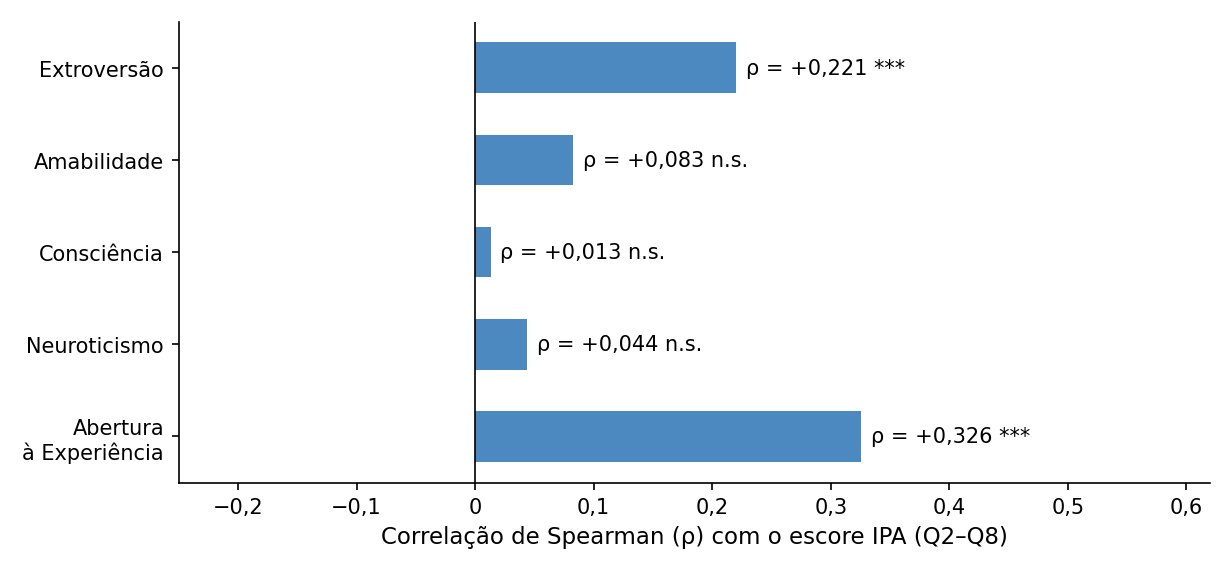
\includegraphics[width=0.8\textwidth]{../resultados/figuras/fig1_spearman_piloto.png}
    \legend{Fonte: dados da pesquisa.}
\end{figure}

\begin{figure}[htb]
    \caption{Estudo piloto: distribuição do escore IPA por nível induzido (\textit{boxplots})}
    \label{fig:boxplots-piloto}
    \centering
    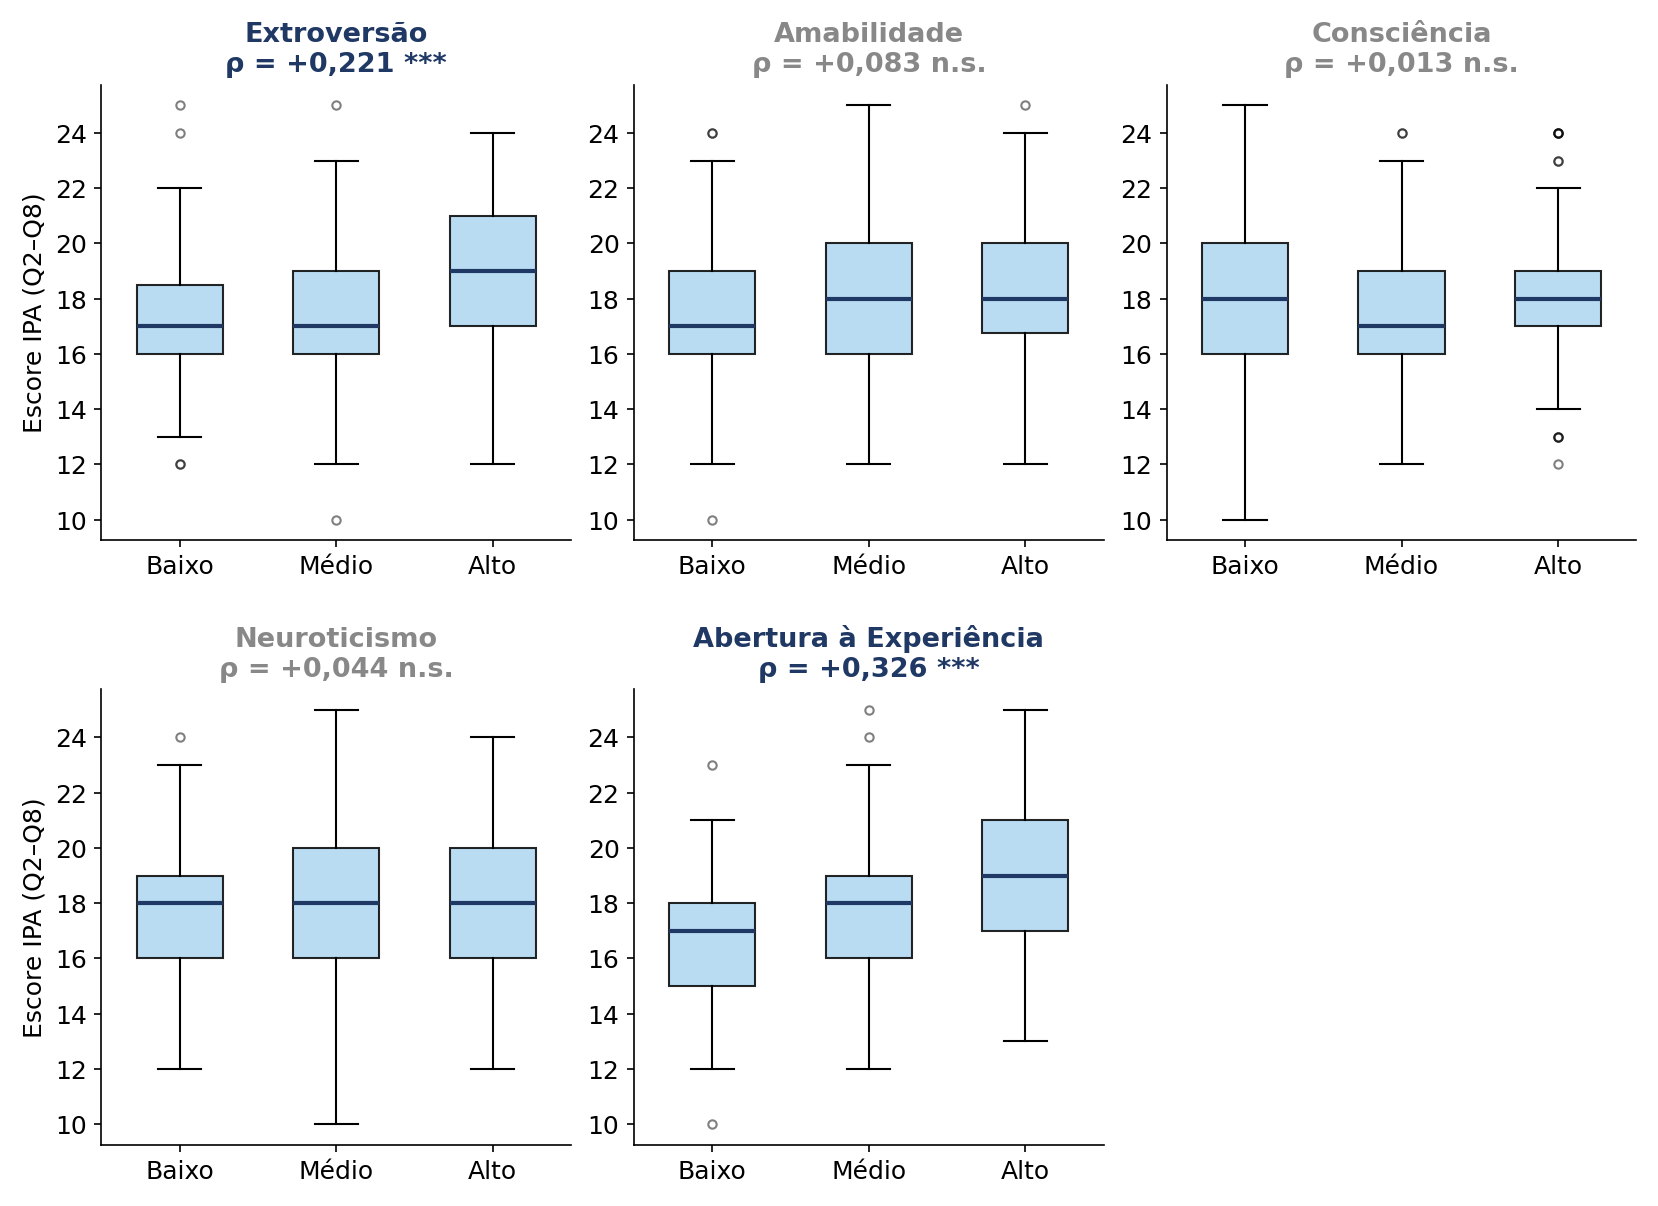
\includegraphics[width=\textwidth]{../resultados/figuras/fig2_boxplots_piloto.png}
    \legend{Fonte: dados da pesquisa.}
\end{figure}

Na regressão OLS com os cinco traços simultâneos (Tabela
\ref{tab:ols-piloto}, Figura \ref{fig:ols-piloto}), o modelo geral obteve
$R^2=0{,}169$; $F(5, 294)=11{,}96$; $p<0{,}001$. Apenas Abertura à
Experiência e Extroversão apresentaram coeficiente estatisticamente
significativo.

\begin{table}[htb]
    \caption{Estudo piloto: regressão OLS, variável dependente: escore IPA (BFI-10, Q2--Q8)}
    \label{tab:ols-piloto}
    \centering
    \begin{tabular}{lcc}
        \toprule
        Traço & Coeficiente & p-valor \\
        \midrule
        Abertura à Experiência & 1,117 & $<$ 0,001 \\
        Extroversão            & 0,717 & $<$ 0,001 \\
        Amabilidade             & 0,261 & 0,145 \\
        Neuroticismo           & 0,179 & 0,335 \\
        Consciência            & 0,069 & 0,705 \\
        \bottomrule
    \end{tabular}
    \legend{Fonte: dados da pesquisa.}
\end{table}

\begin{figure}[htb]
    \caption{Estudo piloto: coeficientes da regressão OLS por traço}
    \label{fig:ols-piloto}
    \centering
    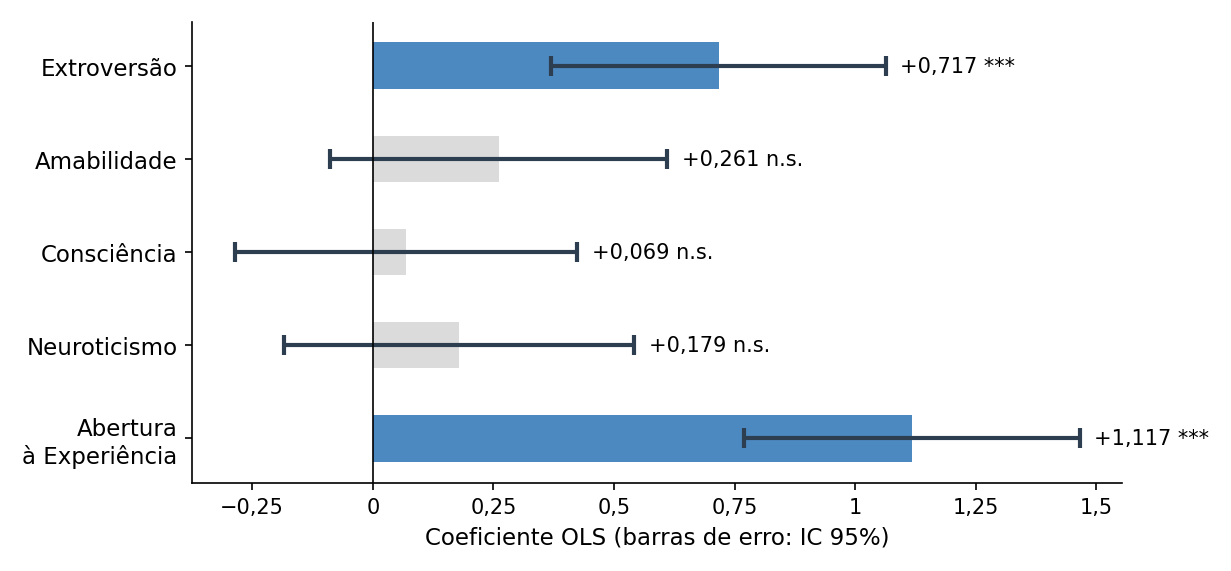
\includegraphics[width=0.8\textwidth]{../resultados/figuras/fig3_ols_piloto.png}
    \legend{Fonte: dados da pesquisa.}
\end{figure}

Esses resultados motivaram tanto a escolha do \texttt{llama3.1:8b} como
modelo principal (seção \ref{sec:selecao-modelo}) quanto a migração para
o BFI-44 como instrumento de checagem de manipulação na análise
principal, reportada a seguir.

\section{Análise principal: Experimento A (BFI-44, multi-traço)}
\label{sec:resultados-exp-a}

\subsection{Checagem de manipulação}
\label{sec:resultados-manipulacao}

A Tabela \ref{tab:manipulacao} apresenta a correlação de Spearman entre o
nível de personalidade induzido (1/2/3) e o escore de autorrelato do
agente no BFI-44, por traço.

\begin{table}[htb]
    \caption{Experimento A: correlação entre nível induzido e autorrelato de personalidade (N=300)}
    \label{tab:manipulacao}
    \centering
    \begin{tabular}{lccc}
        \toprule
        Traço & $\rho$ & p-valor & Avaliação \\
        \midrule
        Extroversão              & 0,929 & $<$ 0,001 & Forte \\
        Abertura à Experiência   & 0,913 & $<$ 0,001 & Forte \\
        Consciência              & 0,879 & $<$ 0,001 & Forte \\
        Neuroticismo             & 0,835 & $<$ 0,001 & Forte \\
        Amabilidade              & 0,813 & $<$ 0,001 & Forte \\
        \bottomrule
    \end{tabular}
    \legend{Fonte: dados da pesquisa.}
\end{table}

\begin{figure}[htb]
    \caption{Experimento A: checagem de manipulação por traço}
    \label{fig:manipulacao}
    \centering
    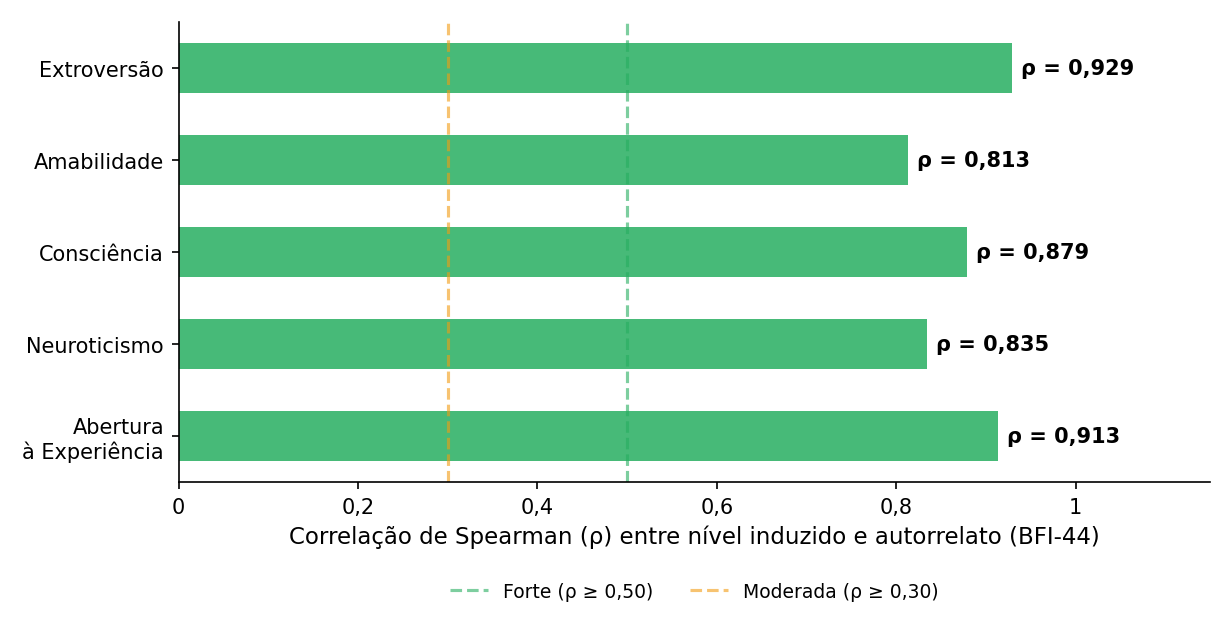
\includegraphics[width=0.8\textwidth]{../resultados/figuras/fig4_manipulacao.png}
    \legend{Fonte: dados da pesquisa.}
\end{figure}

Todos os cinco traços foram incorporados de forma forte e
estatisticamente significativa ($\rho$ de 0,813 a 0,929; Tabela
\ref{tab:manipulacao} e Figura \ref{fig:manipulacao}), uma faixa mais
alta e mais uniforme do que no estudo piloto com BFI-10 (0,410 a 0,838,
Tabela \ref{tab:manipulacao-piloto}).

\subsection{Correlação entre os traços autorrelatados}
\label{sec:resultados-intercorrelacao}

O \texttt{llama3.1:8b} produziu pouca correlação entre os traços
autorrelatados. A
correlação média, em módulo, entre os escores de autorrelato dos 10 pares
de traços foi de 0,110; a maior foi entre Extroversão e Amabilidade
($\rho$ = 0,281), e 4 dos 10 pares tiveram correlação significativa. Como
os níveis induzidos são independentes por construção, essas correlações
vêm do próprio modelo. Mesmo assim, cada nível induzido se reflete
sobretudo no autorrelato do próprio traço: a correlação com o próprio
autorrelato vai de 0,813 a 0,929 (Tabela \ref{tab:manipulacao}), enquanto
a maior correlação entre o nível induzido de um traço e o autorrelato de
outro foi de 0,231 (Amabilidade induzida e Consciência autorrelatada).
Abertura à Experiência foi o traço menos afetado pelos demais: nenhum
outro nível induzido teve correlação significativa com a Abertura
autorrelatada (a maior foi 0,107, com Extroversão; p = 0,063), e incluir
os outros quatro níveis induzidos acrescenta apenas 0,011 ao $R^2$ do
autorrelato de Abertura explicado pelo seu próprio nível. Esse resultado
é compatível com um efeito de Abertura à Experiência sobre o IPA,
reportado a seguir, que não decorre da indução de outro traço.

\subsection{Distribuição do perfil de investidor (IPA)}

A Tabela \ref{tab:distribuicao-ipa} mostra a distribuição do perfil de
investidor obtido no Experimento A.

\begin{table}[htb]
    \caption{Experimento A: distribuição do perfil IPA (N=300)}
    \label{tab:distribuicao-ipa}
    \centering
    \begin{tabular}{lcc}
        \toprule
        Perfil & N & \% \\
        \midrule
        Conservador & 11  & 3,7\%  \\
        Moderado    & 247 & 82,3\% \\
        Arrojado    & 42  & 14,0\% \\
        \bottomrule
    \end{tabular}
    \legend{Fonte: dados da pesquisa. Escore IPA (Q2--Q8): média = 17,58; desvio padrão = 2,72.}
\end{table}

\subsection{Correlação de Spearman: nível induzido \texorpdfstring{$\times$}{x} escore IPA}

A Tabela \ref{tab:spearman-ipa} e as Figuras \ref{fig:spearman} e
\ref{fig:boxplots} apresentam a correlação entre o nível induzido e o
escore do IPA, por traço.

\begin{table}[htb]
    \caption{Experimento A: correlação de Spearman entre nível induzido e escore IPA (N=300)}
    \label{tab:spearman-ipa}
    \centering
    \begin{tabular}{lcc}
        \toprule
        Traço & $\rho$ & p-valor \\
        \midrule
        Abertura à Experiência & 0,530 & $<$ 0,001 \\
        Extroversão            & 0,340 & $<$ 0,001 \\
        Consciência            & 0,206 & $<$ 0,001 \\
        Neuroticismo           & 0,136 & 0,018 \\
        Amabilidade             & 0,051 & 0,376 \\
        \bottomrule
    \end{tabular}
    \legend{Fonte: dados da pesquisa.}
\end{table}

\begin{figure}[htb]
    \caption{Experimento A: correlação de Spearman entre nível induzido e escore IPA}
    \label{fig:spearman}
    \centering
    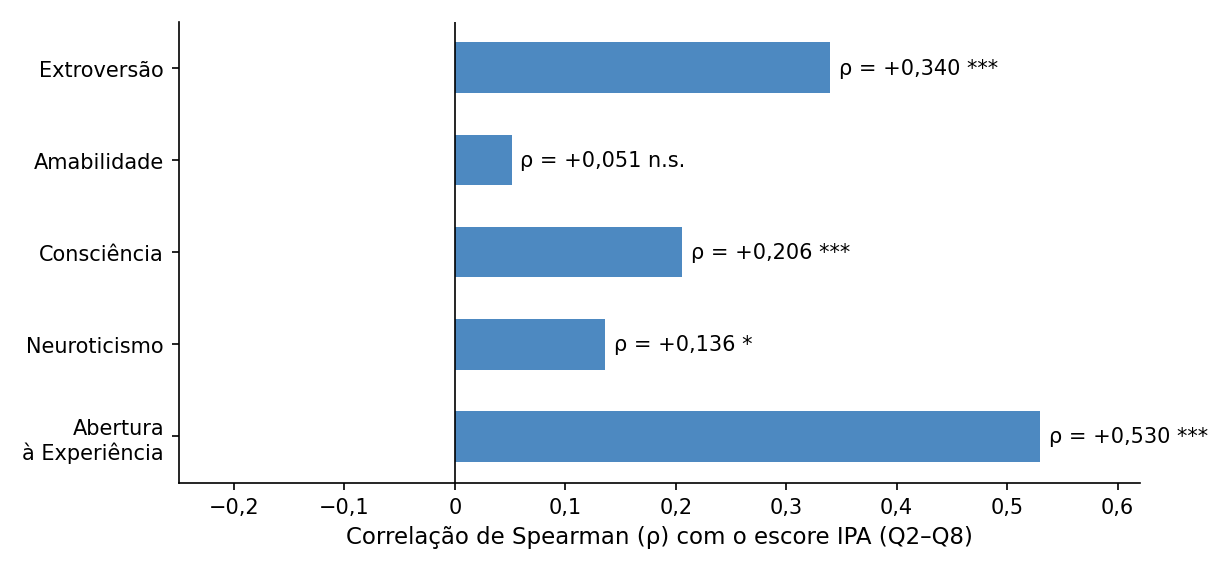
\includegraphics[width=0.8\textwidth]{../resultados/figuras/fig1_spearman.png}
    \legend{Fonte: dados da pesquisa.}
\end{figure}

\begin{figure}[htb]
    \caption{Experimento A: distribuição do escore IPA por nível induzido (\textit{boxplots})}
    \label{fig:boxplots}
    \centering
    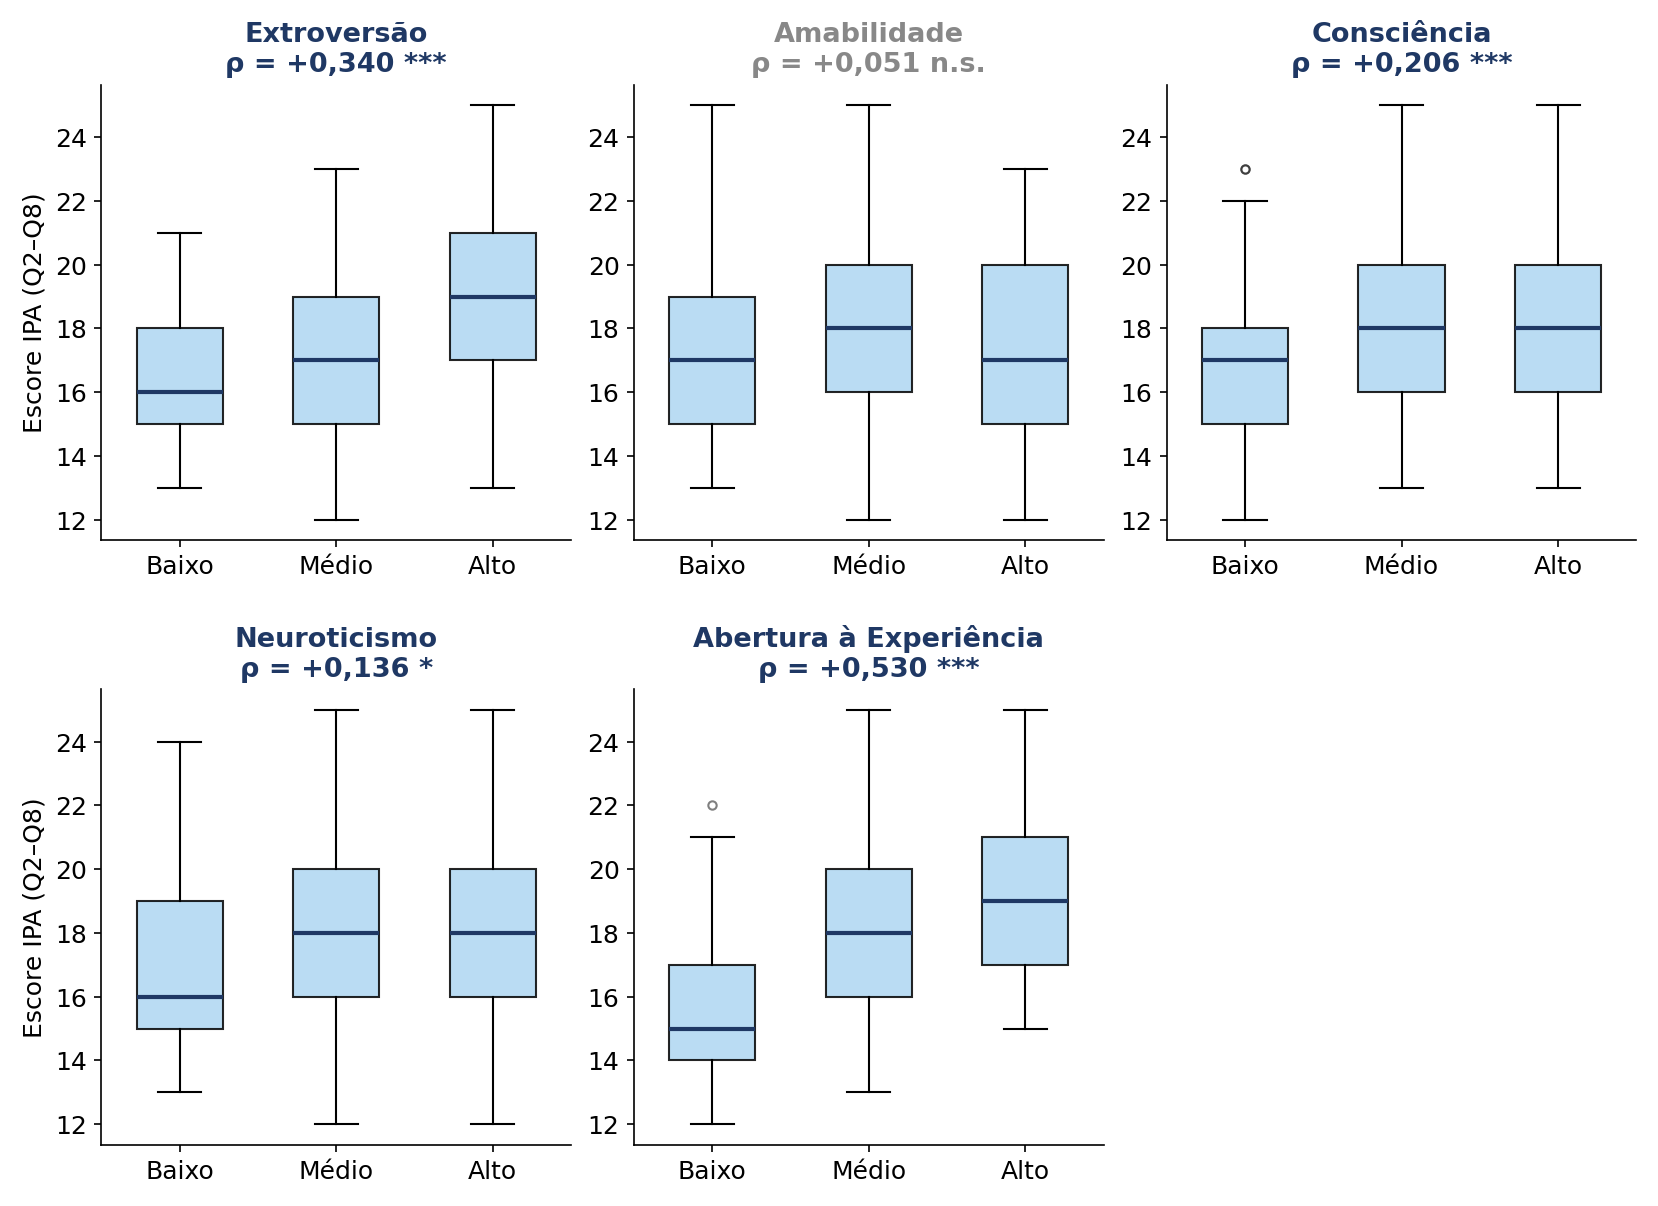
\includegraphics[width=\textwidth]{../resultados/figuras/fig2_boxplots.png}
    \legend{Fonte: dados da pesquisa.}
\end{figure}

\subsection{Regressão OLS com os cinco traços simultâneos}

Os resultados da regressão estão na Tabela \ref{tab:ols} e na Figura
\ref{fig:ols}. Modelo geral: $R^2=0{,}459$; $F(5, 294)=49{,}85$; $p<0{,}001$.

\begin{table}[htb]
    \caption{Experimento A: regressão OLS, variável dependente: escore IPA (Q2--Q8)}
    \label{tab:ols}
    \centering
    \begin{tabular}{lcc}
        \toprule
        Traço & Coeficiente & p-valor \\
        \midrule
        Abertura à Experiência & 1,716 & $<$ 0,001 \\
        Extroversão            & 1,189 & $<$ 0,001 \\
        Consciência            & 0,750 & $<$ 0,001 \\
        Neuroticismo           & 0,407 & 0,006 \\
        Amabilidade             & 0,094 & 0,511 \\
        \bottomrule
    \end{tabular}
    \legend{Fonte: dados da pesquisa.}
\end{table}

\begin{figure}[htb]
    \caption{Experimento A: coeficientes da regressão OLS por traço}
    \label{fig:ols}
    \centering
    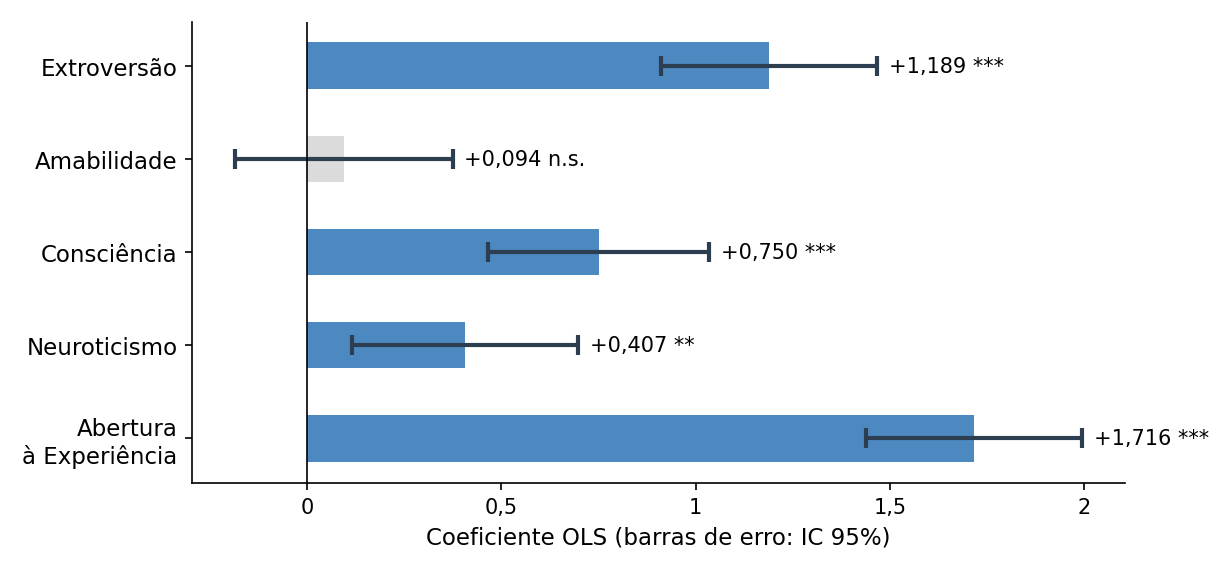
\includegraphics[width=0.8\textwidth]{../resultados/figuras/fig3_ols.png}
    \legend{Fonte: dados da pesquisa.}
\end{figure}

Controlando o efeito dos outros quatro traços, cada passo de nível (de
Baixo para Médio ou de Médio para Alto) em Abertura à Experiência
corresponde, em média, a um acréscimo de 1,716 ponto no escore IPA, o
maior coeficiente entre os cinco traços. Extroversão, Consciência e
Neuroticismo têm coeficientes positivos e estatisticamente significativos
(1,189, 0,750 e 0,407 ponto por passo de nível, respectivamente),
enquanto Amabilidade não apresenta efeito distinguível de zero
(coeficiente de 0,094; $p=0{,}511$). O modelo como um todo explica 45,9\% da variância do
escore IPA, quase o triplo do $R^2$ obtido no estudo piloto com BFI-10
(16,9\%, Tabela \ref{tab:ols-piloto}). Quatro dos cinco traços atingem
significância estatística nesta análise, contra dois no estudo piloto; a
seção seguinte (Experimento B) verifica até que ponto esses quatro
efeitos dependem do desenho de indução simultânea.

\section{Experimento B: traço dominante}
\label{sec:resultados-exp-b}

O Experimento B foi conduzido para verificar se induzir os cinco traços
do Big Five ao mesmo tempo no mesmo agente, como no Experimento A, dilui
ou confunde o sinal de cada traço individual, em comparação com a
indução de apenas um traço por vez. Para testar isso de forma
controlada, o Experimento B usa o mesmo modelo e instrumento do
Experimento A, mudando apenas o desenho de indução: cada agente tem
apenas um dos cinco traços sorteado para variar (o ``traço dominante''),
com os outros quatro fixos em ``Médio'' (a seção \ref{sec:exp-a-b}
descreve o raciocínio metodológico completo; a interpretação dos números
a seguir está no Capítulo \ref{cap:discussao}, seção
\ref{sec:discussao-exp-b}). A Tabela \ref{tab:manipulacao-exp-b} reporta
a checagem de manipulação, calculada apenas entre os agentes em que
aquele traço era o dominante (por isso o N varia por linha, de 49 a 69),
lado a lado com o valor correspondente do Experimento A.

\begin{table}[htb]
    \caption{Checagem de manipulação: Experimento A (todos os traços variando) vs. Experimento B (só o traço dominante variando)}
    \label{tab:manipulacao-exp-b}
    \centering
    \begin{tabular}{lcccc}
        \toprule
        Traço & $\rho$ Exp. A & $\rho$ Exp. B & N (Exp. B) & p-valor (Exp. B) \\
        \midrule
        Extroversão              & 0,929 & 0,930 & 57 & $<$ 0,001 \\
        Abertura à Experiência   & 0,913 & 0,928 & 49 & $<$ 0,001 \\
        Consciência              & 0,879 & 0,896 & 63 & $<$ 0,001 \\
        Neuroticismo             & 0,835 & 0,840 & 69 & $<$ 0,001 \\
        Amabilidade              & 0,813 & 0,837 & 62 & $<$ 0,001 \\
        \bottomrule
    \end{tabular}
    \legend{Fonte: dados da pesquisa. Coluna ``Exp. B'' calculada apenas entre os agentes em que o traço da linha era o traço dominante sorteado.}
\end{table}

\begin{figure}[htb]
    \caption{Checagem de manipulação: Experimento A vs. Experimento B, por traço}
    \label{fig:exp-ab-manipulacao}
    \centering
    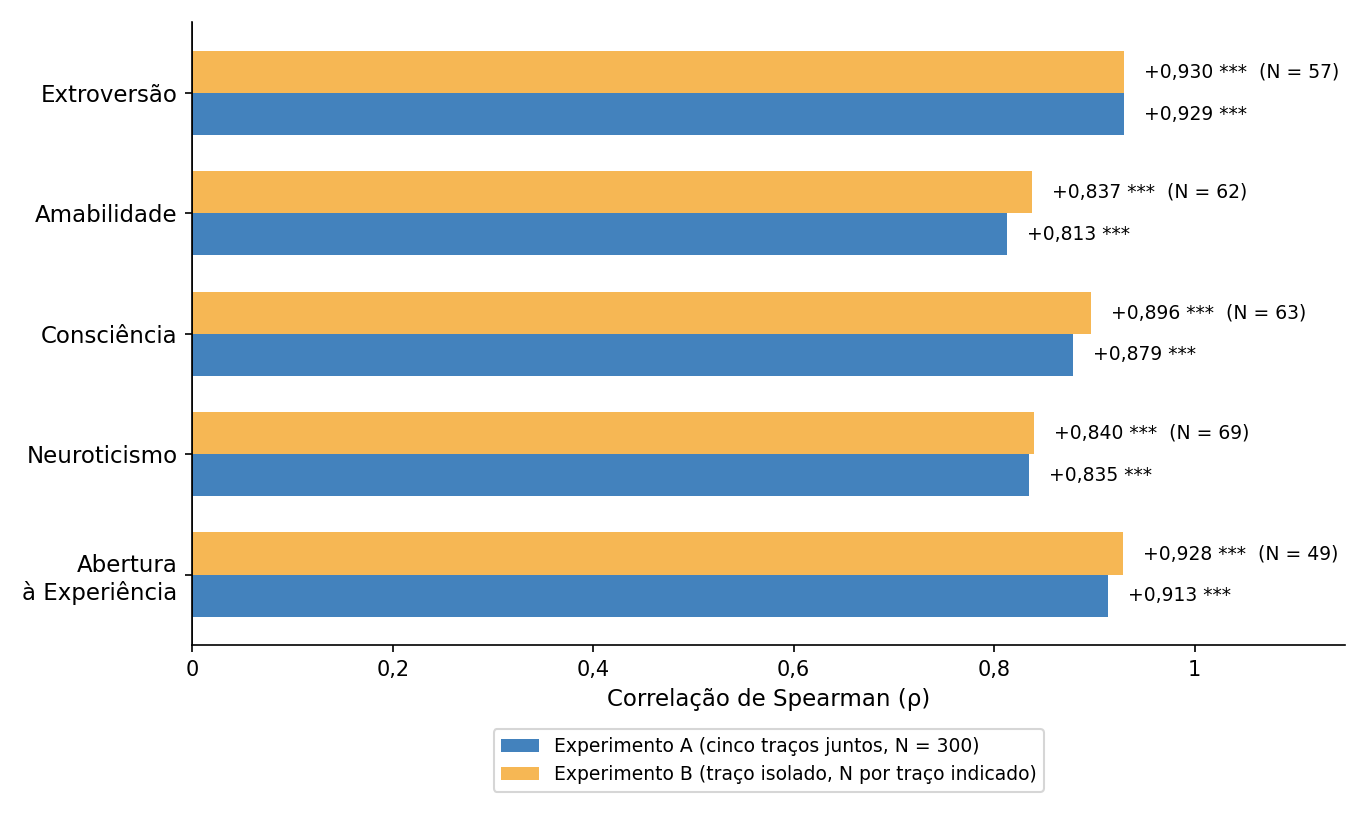
\includegraphics[width=0.85\textwidth]{../resultados/figuras/fig8_exp_ab_manipulacao.png}
    \legend{Fonte: dados da pesquisa.}
\end{figure}

Na Figura \ref{fig:exp-ab-manipulacao}, os valores dos dois experimentos
são praticamente iguais em todos os traços, entre 0,8 e 0,95.

A Tabela \ref{tab:ipa-exp-b} reporta a correlação entre nível induzido e
escore do IPA, na mesma estratificação, lado a lado com o Experimento A.

\begin{table}[htb]
    \caption{Correlação com o escore IPA: Experimento A (todos os traços) vs. Experimento B (traço dominante)}
    \label{tab:ipa-exp-b}
    \centering
    \begin{tabular}{lcccc}
        \toprule
        Traço & $\rho$ Exp. A & $\rho$ Exp. B & N (Exp. B) & p-valor (Exp. B) \\
        \midrule
        Abertura à Experiência   & 0,530  & 0,792  & 49 & $<$ 0,001 \\
        Extroversão              & 0,340  & 0,242  & 57 & 0,070 \\
        Consciência              & 0,206  & 0,153  & 63 & 0,232 \\
        Neuroticismo             & 0,136  & $-$0,116 & 69 & 0,344 \\
        Amabilidade              & 0,051  & $-$0,006 & 62 & 0,966 \\
        \bottomrule
    \end{tabular}
    \legend{Fonte: dados da pesquisa. Coluna ``Exp. B'' calculada apenas entre os agentes em que o traço da linha era o traço dominante sorteado.}
\end{table}

\begin{figure}[htb]
    \caption{Correlação com o escore IPA: Experimento A vs. Experimento B, por traço}
    \label{fig:exp-ab-ipa}
    \centering
    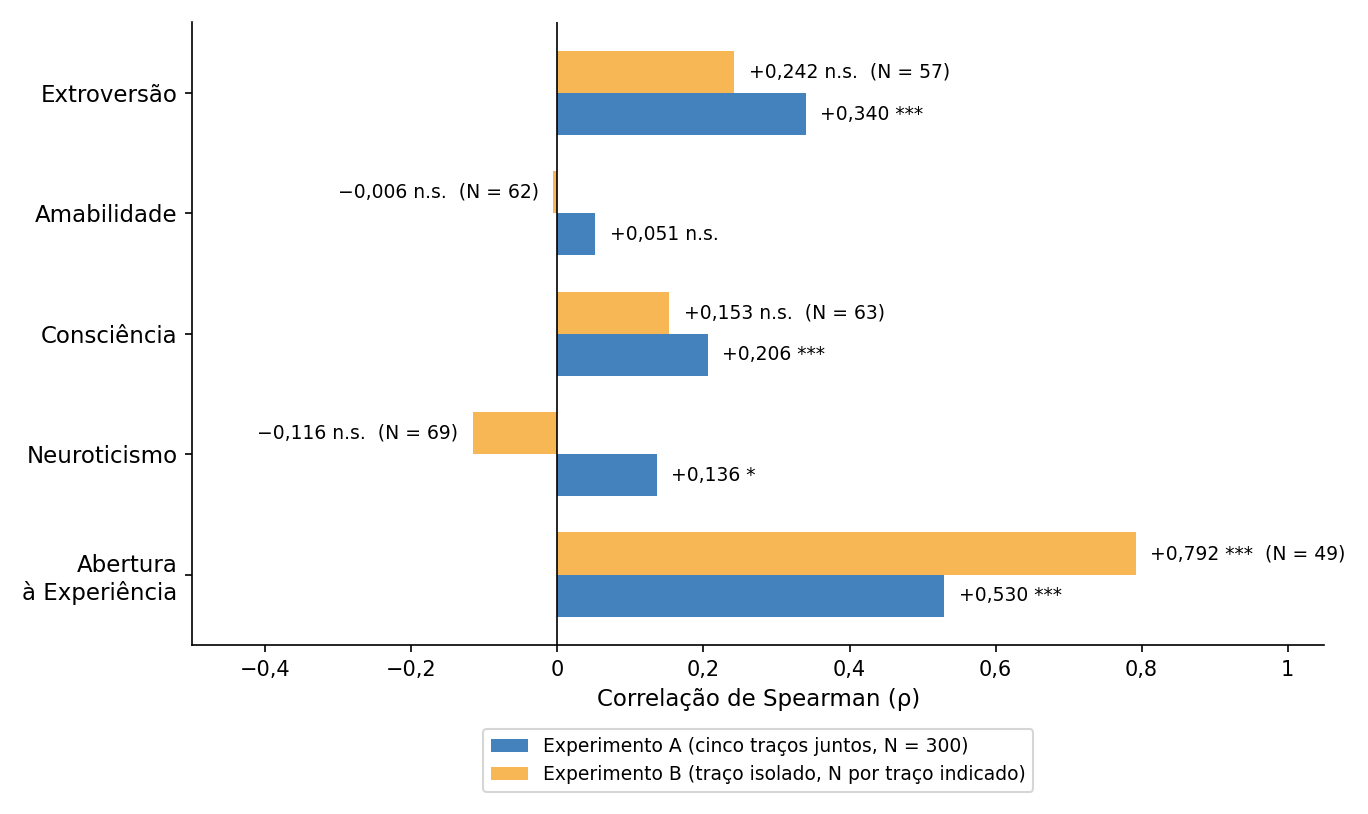
\includegraphics[width=0.85\textwidth]{../resultados/figuras/fig9_exp_ab_ipa.png}
    \legend{Fonte: dados da pesquisa.}
\end{figure}

Ao contrário da Figura \ref{fig:exp-ab-manipulacao}, na Figura
\ref{fig:exp-ab-ipa} os valores dos dois experimentos não são
parecidos em todos os traços: em Abertura à Experiência, a correlação é
maior no Experimento B; nos outros quatro traços, é menor no Experimento
B, e em Neuroticismo e Amabilidade passa a ser negativa.

A checagem de manipulação (Tabela \ref{tab:manipulacao-exp-b}) é
comparável entre os dois desenhos em todos os cinco traços, sem indício
de que a indução simultânea enfraqueça a manipulação. Já a correlação
com o escore IPA (Tabela \ref{tab:ipa-exp-b}) mostra um padrão diferente
por traço: Abertura à Experiência permanece significativa e com
correlação mais alta no Experimento B ($\rho=0{,}792$ contra 0,530); os
outros quatro traços não atingem significância estatística no
Experimento B, com Neuroticismo e Amabilidade invertendo o sinal
(positivo no Experimento A, negativo no B). A interpretação desse
padrão, incluindo o papel do N bem menor por traço no Experimento B
(49 a 69, contra 300 no Experimento A), é discutida no Capítulo
\ref{cap:discussao}.

\section{Análise de robustez e generalização}
\label{sec:resultados-robustez}

Esta seção reporta as repetições do Experimento A descritas na seção
\ref{sec:metodo-robustez}. Em todas as tabelas, o escore IPA é o das
perguntas 2 a 8 e os coeficientes são os da regressão OLS com os cinco
níveis induzidos, com a mesma notação de significância usada no restante
do trabalho (* $p<0{,}05$; ** $p<0{,}01$; *** $p<0{,}001$; n.s. para
$p \geq 0{,}05$). A faixa de manipulação é o menor e o maior $\rho$ entre
nível induzido e autorrelato (BFI-44) entre os cinco traços.

\subsection{Sensibilidade à temperatura}

As três novas rodadas foram concluídas com 300 agentes cada, com BFI-44 válido em
todos e IPA válido em 299 (temperaturas 0,0 e 0,3) e 300 (temperatura
1,0) agentes. A Tabela \ref{tab:robustez-temperatura} compara as quatro
temperaturas.

\begin{table}[htb]
    \caption{Experimento A em quatro temperaturas (\texttt{llama3.1:8b}, N=300, mesmos perfis)}
    \label{tab:robustez-temperatura}
    \centering
    \footnotesize
    \setlength{\tabcolsep}{4pt}
    \begin{tabular}{>{\raggedright\arraybackslash}p{3.4cm}cccc}
        \toprule
        Indicador & 0,0 & 0,3 & 0,7 (Exp. A) & 1,0 \\
        \midrule
        Perfis IPA: Conservador / Moderado / Arrojado (\%) & 2,0 / 86,6 / 11,4 & 3,7 / 84,9 / 11,4 & 3,7 / 82,3 / 14,0 & 4,0 / 81,0 / 15,0 \\
        Escore IPA: média (desvio padrão) & 17,05 (2,41) & 17,09 (2,47) & 17,58 (2,72) & 17,67 (2,77) \\
        Manipulação: faixa de $\rho$ & 0,873 a 0,946 & 0,859 a 0,938 & 0,813 a 0,929 & 0,809 a 0,920 \\
        $R^2$ da regressão OLS & 0,707 & 0,643 & 0,459 & 0,449 \\
        \midrule
        Coef. Abertura à Experiência & 1,767*** & 1,932*** & 1,716*** & 1,686*** \\
        Coef. Extroversão & 1,595*** & 1,273*** & 1,189*** & 1,253*** \\
        Coef. Consciência & 0,429*** & 0,486*** & 0,750*** & 0,301* \\
        Coef. Neuroticismo & 0,419*** & 0,278* & 0,407** & 0,744*** \\
        Coef. Amabilidade & 0,359*** & 0,344** & 0,094 n.s. & 0,246 n.s. \\
        \bottomrule
    \end{tabular}
    \legend{Fonte: dados da pesquisa.}
\end{table}

Abertura à Experiência teve o maior coeficiente nas quatro temperaturas
(de 1,686 a 1,932), sempre com $p<0{,}001$, e Extroversão o segundo maior
(de 1,189 a 1,595), também sempre com $p<0{,}001$. Abaixo de 0,7, a
manipulação fica mais fiel e o $R^2$ sobe (0,643 em 0,3 e 0,707 em 0,0), enquanto em 1,0 o resultado fica
próximo do obtido em 0,7 ($R^2=0{,}449$). Os três traços de efeito menor
oscilam entre temperaturas: o coeficiente de Consciência vai de 0,301
(1,0) a 0,750 (0,7), o de Neuroticismo vai de 0,278 (0,3) a 0,744 (1,0),
e Amabilidade só é significativa em 0,0 e 0,3.

A temperatura 0,0 não tornou a geração totalmente determinística. Como a
pergunta 1 do IPA não entra no \textit{prompt}, agentes com a mesma
combinação de níveis recebem \textit{prompts} idênticos. Entre as 87
combinações de níveis que aparecem em mais de um agente, o escore IPA foi
idêntico em todos os agentes da combinação em 87,4\% delas com
temperatura 0,0, contra 6,9\% com temperatura 0,7.

Como os perfis são os mesmos do Experimento A, cada agente pode ser
comparado consigo mesmo entre temperaturas (Tabela
\ref{tab:robustez-temperatura-pareada}). O mesmo agente recebeu o mesmo
perfil de investidor em 77,3\% a 82,9\% dos casos, com a menor
concordância na temperatura 1,0.

\begin{table}[htb]
    \caption{Comparação agente a agente com o Experimento A (temperatura 0,7)}
    \label{tab:robustez-temperatura-pareada}
    \centering
    \begin{tabular}{lccc}
        \toprule
        Temperatura & Pares & $\rho$ do escore IPA & Mesmo perfil IPA (\%) \\
        \midrule
        0,0 & 299 & 0,620*** & 82,9 \\
        0,3 & 299 & 0,583*** & 82,9 \\
        1,0 & 300 & 0,526*** & 77,3 \\
        \bottomrule
    \end{tabular}
    \legend{Fonte: dados da pesquisa.}
\end{table}

\subsection{Novo sorteio de perfis}

O novo sorteio (semente 456) também ficou equilibrado: cada nível de cada
traço recebeu entre 88 e 117 dos 300 agentes, sem desvio significativo da
distribuição uniforme ($\chi^2$, p $\geq$ 0,101), e os níveis sorteados
ficaram independentes entre os traços ($|\rho| \leq$ 0,087). O BFI-44 foi
válido nos 300 agentes e o IPA em 298. A Tabela \ref{tab:robustez-seed}
compara os dois sorteios.

\begin{table}[htb]
    \caption{Experimento A com dois sorteios de perfis (\texttt{llama3.1:8b}, temperatura 0,7)}
    \label{tab:robustez-seed}
    \centering
    \begin{tabular}{lcc}
        \toprule
        Indicador & Semente 123 (Exp. A) & Semente 456 \\
        \midrule
        Perfis IPA: C / M / A (\%) & 3,7 / 82,3 / 14,0 & 6,7 / 80,2 / 13,1 \\
        Escore IPA: média (desvio padrão) & 17,58 (2,72) & 17,50 (2,77) \\
        Manipulação: faixa de $\rho$ & 0,813 a 0,929 & 0,823 a 0,928 \\
        $R^2$ da regressão OLS & 0,459 & 0,526 \\
        \midrule
        Coef. Abertura à Experiência & 1,716*** & 2,106*** \\
        Coef. Extroversão & 1,189*** & 1,293*** \\
        Coef. Consciência & 0,750*** & 0,048 n.s. \\
        Coef. Neuroticismo & 0,407** & $-$0,092 n.s. \\
        Coef. Amabilidade & 0,094 n.s. & 0,169 n.s. \\
        \bottomrule
    \end{tabular}
    \legend{Fonte: dados da pesquisa. C = Conservador; M = Moderado; A = Arrojado.}
\end{table}

Abertura à Experiência e Extroversão se repetem no novo sorteio, com
coeficientes de tamanho semelhante ou maior (2,106 e 1,293). Consciência
e Neuroticismo, significativos no Experimento A, ficam próximos de zero e
sem significância com outro sorteio de perfis, e Amabilidade continua sem
efeito.

\subsection{Outros modelos de linguagem}

As rodadas com os três modelos abertos foram concluídas com 300 agentes cada, com
os mesmos perfis do Experimento A. A taxa de respostas válidas variou
entre os modelos: o \texttt{gemma3:12b} teve BFI-44 e IPA válidos nos 300
agentes; o \texttt{mistral:7b}, BFI-44 válido em 294 e IPA em 300; e o
\texttt{qwen2.5:7b}, BFI-44 válido em 286 e IPA em 257, de modo que a
análise desse modelo usa os 245 agentes com os dois questionários
válidos. A Tabela \ref{tab:robustez-modelos} reporta os resultados.

\begin{table}[htb]
    \caption{Experimento A em quatro modelos abertos (temperatura 0,7, mesmos perfis)}
    \label{tab:robustez-modelos}
    \centering
    \footnotesize
    \setlength{\tabcolsep}{4pt}
    \begin{tabular}{>{\raggedright\arraybackslash}p{3.3cm}>{\centering\arraybackslash}p{2.5cm}>{\centering\arraybackslash}p{2.5cm}>{\centering\arraybackslash}p{2.5cm}>{\centering\arraybackslash}p{2.5cm}}
        \toprule
        Indicador & \texttt{llama3.1:8b} (Exp. A) & \texttt{qwen2.5:7b} & \texttt{mistral:7b} & \texttt{gemma3:12b} \\
        \midrule
        Agentes na análise & 300 & 245 & 294 & 300 \\
        Perfis IPA: C / M / A (\%) & 3,7 / 82,3 / 14,0 & 4,5 / 51,0 / 44,5 & 0,0 / 8,5 / 91,5 & 24,0 / 59,3 / 16,7 \\
        Escore IPA: média (desvio padrão) & 17,58 (2,72) & 19,48 (4,34) & 22,86 (1,11) & 15,77 (3,89) \\
        Manipulação: faixa de $\rho$ & 0,813 a 0,929 & 0,846 a 0,914 & 0,872 a 0,939 & 0,943 a 0,957 \\
        $R^2$ da regressão OLS & 0,459 & 0,796 & 0,383 & 0,648 \\
        \midrule
        Coef. Abertura à Experiência & 1,716*** & 4,643*** & 0,632*** & 2,622*** \\
        Coef. Extroversão & 1,189*** & 1,551*** & 0,391*** & 2,697*** \\
        Coef. Consciência & 0,750*** & $-$0,426** & 0,034 n.s. & 0,534** \\
        Coef. Neuroticismo & 0,407** & 0,322* & 0,285*** & $-$0,125 n.s. \\
        Coef. Amabilidade & 0,094 n.s. & $-$0,317* & $-$0,287*** & $-$0,193 n.s. \\
        \bottomrule
    \end{tabular}
    \legend{Fonte: dados da pesquisa. C = Conservador; M = Moderado; A = Arrojado.}
\end{table}

A indução de personalidade funcionou nos quatro modelos: nos três
modelos adicionais, o menor $\rho$ de manipulação entre os cinco traços
(0,846 a 0,943) ficou acima do menor $\rho$ do \texttt{llama3.1:8b}
(0,813). Abertura à
Experiência e Extroversão elevam o escore IPA nos quatro, sempre com
$p<0{,}001$, embora o tamanho do efeito varie bastante: no
\texttt{qwen2.5:7b}, o coeficiente de Abertura é cerca de 2,7 vezes o do
\texttt{llama3.1:8b} (4,643 contra 1,716), e no \texttt{mistral:7b} é bem
menor (0,632). Os outros três traços não se repetem: Consciência é
positiva no \texttt{llama3.1:8b} e no \texttt{gemma3:12b}, negativa no
\texttt{qwen2.5:7b} e nula no \texttt{mistral:7b}; Neuroticismo é
positivo em três modelos e nulo no \texttt{gemma3:12b}; e Amabilidade,
nula no \texttt{llama3.1:8b}, é negativa e significativa no
\texttt{qwen2.5:7b} e no \texttt{mistral:7b}.

A distribuição dos perfis de investidor, por sua vez, depende fortemente do modelo.
O \texttt{mistral:7b} classificou 91,5\% dos agentes como Arrojado, com
escore pouco variável (desvio padrão de 1,11), enquanto o
\texttt{llama3.1:8b} classificou 82,3\% como Moderado e o
\texttt{gemma3:12b} teve a maior proporção de Conservadores (24,0\%). A
comparação agente a agente com o \texttt{llama3.1:8b} (Tabela
\ref{tab:robustez-modelos-pareada}) mostra que, com o mesmo perfil de
personalidade, o perfil de investidor coincide em 20,3\% a 62,0\% dos
agentes, conforme o modelo.

\begin{table}[htb]
    \caption{Comparação agente a agente com o \texttt{llama3.1:8b} (Experimento A)}
    \label{tab:robustez-modelos-pareada}
    \centering
    \begin{tabular}{lccc}
        \toprule
        Modelo & Pares & $\rho$ do escore IPA & Mesmo perfil IPA (\%) \\
        \midrule
        \texttt{qwen2.5:7b}  & 257 & 0,559*** & 54,5 \\
        \texttt{mistral:7b}  & 300 & 0,348*** & 20,3 \\
        \texttt{gemma3:12b}  & 300 & 0,560*** & 62,0 \\
        \bottomrule
    \end{tabular}
    \legend{Fonte: dados da pesquisa. Pares: agentes com IPA válido nas duas rodadas.}
\end{table}

Os dois modelos Nemotron, rodados como teste exploratório com N=30
(Tabela \ref{tab:robustez-nemotron}), tiveram BFI-44 e IPA válidos nos 30
agentes. Eles seguiram a indução com fidelidade ainda maior (faixa de
manipulação de 0,918 a 0,990) e responderam ao IPA de forma muito mais
extrema que o \texttt{llama3.1:8b}: o desvio padrão do escore IPA é quase
o triplo, e os agentes se distribuem entre Conservador e Arrojado em vez
de se concentrarem em Moderado. Abertura à Experiência e Extroversão
também elevam o escore IPA nos dois modelos, com Abertura como o maior
efeito positivo. No Nemotron 3 Ultra, Amabilidade aparece com efeito
negativo ($-$3,356), o que não ocorre no \texttt{llama3.1:8b}. Com N=30,
esses resultados indicam apenas a direção dos efeitos, não seu tamanho.

\begin{table}[htb]
    \caption{Teste exploratório com os modelos Nemotron (N=30, mesmos perfis dos 30 primeiros agentes do Experimento A)}
    \label{tab:robustez-nemotron}
    \centering
    \footnotesize
    \begin{tabular}{>{\raggedright\arraybackslash}p{4.2cm}>{\centering\arraybackslash}p{3.0cm}>{\centering\arraybackslash}p{3.0cm}>{\centering\arraybackslash}p{3.0cm}}
        \toprule
        Indicador & \texttt{llama3.1:8b} (30 primeiros, Exp. A) & Nemotron 3.5 Super & Nemotron 3 Ultra \\
        \midrule
        Perfis IPA: C / M / A (\%) & 3,3 / 83,3 / 13,3 & 56,7 / 13,3 / 30,0 & 40,0 / 20,0 / 40,0 \\
        Escore IPA: média (desvio padrão) & 18,00 (2,67) & 15,07 (7,71) & 16,83 (7,27) \\
        Manipulação: faixa de $\rho$ & 0,776 a 0,937 & 0,918 a 0,990 & 0,925 a 0,966 \\
        $R^2$ da regressão OLS & 0,455 & 0,659 & 0,799 \\
        \midrule
        Coef. Abertura à Experiência & 1,637** & 6,096*** & 6,751*** \\
        Coef. Extroversão & 1,322* & 4,035** & 2,060* \\
        Coef. Consciência & 0,106 n.s. & 1,443 n.s. & 1,274 n.s. \\
        Coef. Neuroticismo & $-$0,270 n.s. & $-$0,541 n.s. & $-$1,543 n.s. \\
        Coef. Amabilidade & 0,497 n.s. & $-$0,622 n.s. & $-$3,356** \\
        Mesmo perfil IPA do \texttt{llama3.1:8b} (\%) & -- & 30,0 & 36,7 \\
        \bottomrule
    \end{tabular}
    \legend{Fonte: dados da pesquisa. C = Conservador; M = Moderado; A = Arrojado.}
\end{table}

\subsection{Síntese}

A Tabela \ref{tab:robustez-sintese} resume, traço a traço, o sinal e a
significância do coeficiente OLS nas oito rodadas com 300 agentes gerados: as quatro
temperaturas, o novo sorteio e os três modelos abertos adicionais.

\begin{table}[htb]
    \caption{Sinal e significância do coeficiente OLS de cada traço nas oito rodadas com 300 agentes gerados}
    \label{tab:robustez-sintese}
    \centering
    \resizebox{\textwidth}{!}{%
    \begin{tabular}{lcccccccc}
        \toprule
        & \multicolumn{4}{c}{\texttt{llama3.1:8b}, temperatura} & \texttt{llama3.1:8b} & & & \\
        \cmidrule(lr){2-5}
        Traço & 0,0 & 0,3 & 0,7 & 1,0 & semente 456 & \texttt{qwen2.5:7b} & \texttt{mistral:7b} & \texttt{gemma3:12b} \\
        \midrule
        Abertura à Experiência & $+$*** & $+$*** & $+$*** & $+$*** & $+$*** & $+$*** & $+$*** & $+$*** \\
        Extroversão            & $+$*** & $+$*** & $+$*** & $+$*** & $+$*** & $+$*** & $+$*** & $+$*** \\
        Consciência            & $+$*** & $+$*** & $+$*** & $+$*   & n.s.   & $-$**  & n.s.   & $+$**  \\
        Neuroticismo           & $+$*** & $+$*   & $+$**  & $+$*** & n.s.   & $+$*   & $+$*** & n.s.   \\
        Amabilidade            & $+$*** & $+$**  & n.s.   & n.s.   & n.s.   & $-$*   & $-$*** & n.s.   \\
        \bottomrule
    \end{tabular}%
    }
    \legend{Fonte: dados da pesquisa (Tabelas \ref{tab:robustez-temperatura}, \ref{tab:robustez-seed} e \ref{tab:robustez-modelos}). A coluna 0,7 corresponde ao Experimento A. Os sinais $+$ e $-$ indicam se o coeficiente OLS é positivo ou negativo; * $p<0{,}05$; ** $p<0{,}01$; *** $p<0{,}001$; n.s.: não significativo ($p\geq0{,}05$).}
\end{table}

\begin{figure}[htb]
    \caption{Coeficientes OLS de cada traço nas oito rodadas com 300 agentes gerados}
    \label{fig:robustez-coeficientes}
    \centering
    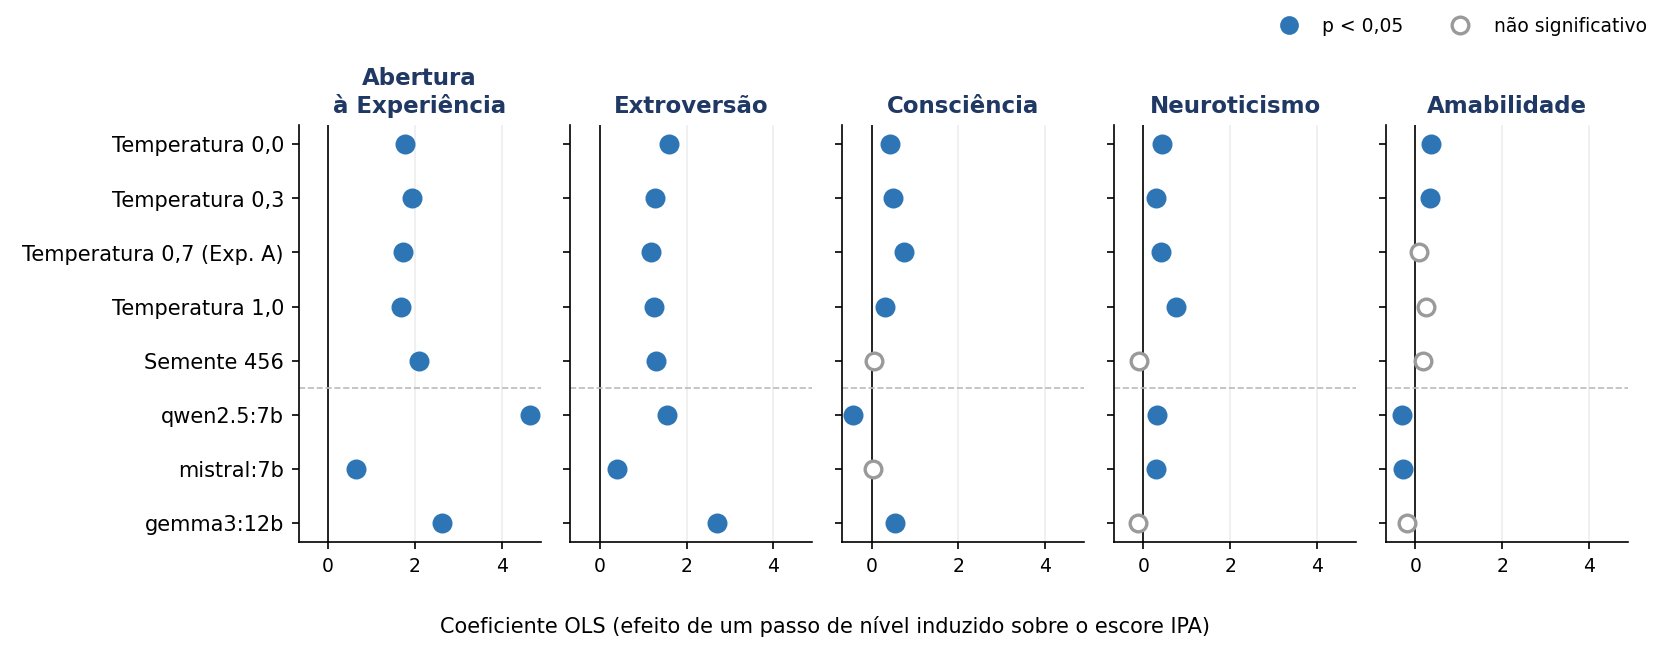
\includegraphics[width=\textwidth]{../resultados/figuras/fig11_robustez_coeficientes.png}
    \legend{Fonte: dados da pesquisa (Tabelas \ref{tab:robustez-temperatura}, \ref{tab:robustez-seed} e \ref{tab:robustez-modelos}). As cinco primeiras linhas usam o \texttt{llama3.1:8b}; a linha tracejada separa as rodadas com outros modelos. Círculos preenchidos: $p<0{,}05$.}
\end{figure}

Abertura à Experiência e Extroversão são positivas e significativas com
$p<0{,}001$ nas oito rodadas (Figura \ref{fig:robustez-coeficientes}). Consciência e Neuroticismo são significativos
na maior parte das rodadas, mas perdem a significância com o novo sorteio
e em parte dos modelos, e Consciência chega a inverter o sinal no
\texttt{qwen2.5:7b}. Amabilidade, sem efeito no Experimento A, aparece
com sinais opostos em diferentes rodadas. A interpretação desse padrão é
feita no Capítulo \ref{cap:discussao}.
